

\chapter{Results and Discussion}
  

  The synthesis of the target ligand molecule \cmpd+{legante} has been achieved joining the molecules resulting from the syntheses of the aliphatic part and of the aromatic part.


\section{Protection of Deoxy\-cholic Acid}

  \begin{SCfigure}[][ht]
    \cmpdref-{da}
    \cmpdref-{amda}
    \centering{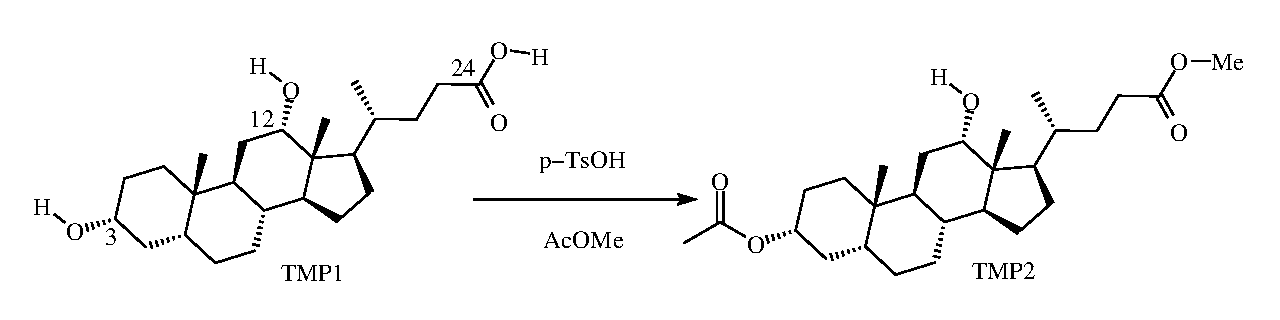
\includegraphics[width=.95\textwidth]{sc/da-amda.eps}}
  \caption{\\ The protection of 7-de\-oxy\-cholic acid \cmpd+{da}.\label{sc:da-amda}}
\end{SCfigure}

\paragraph{Strategy Synthesis}

  As anticipated at page \pageref{dodici}, in order to obtain the maximum chirality transfer to a substituent by the de\-oxy\-cholic group this substituent should be bonded to the alcoholic group on C-12, which is inside the cavity of the 7-de\-oxy\-cholic acid. It's necessary to protect the alcoholic functionality on C-3 because of its competing reactivity and the acidic group to block its unwanted reactivity. Fortunately this protection can be performed in a one-step procedure \cite{CHIN:CHIN199646207} %The commercially available de\-oxy\-cholic acid \cmpd{da} was protected in position 3 and 24 
  using a transesterification with methyl acetate. This selective protection is made possible by the different reactivity of the alcoholic groups at the different positions: hydroxilic group on C-3 is more accessible (an equatorial position) while the one on C-12 is in a more hindered %crowded - Leo
 position (axial). 7-Deoxy\-cholic acid \cmpd+{da} was heated in presence of \p-toluenesulfonic acid using methyl acetate as solvent. 
\paragraph{Results and Characterization}
  The reaction mixture was washed, extracted and purified by column chromatography obtaining protected de\-oxy\-cholic ester \cmpd+{amda} in a 69 \% yield.

  The $^{1}$H-NMR spectrum of protected de\-oxy\-cholic ester \cmpd+{amda} is reported in Figure \ref{sp:amda} and peaks data are reported in Subsection \ref{sec:sperimentale-amda}.
  In the $^{1}$H-NMR spectrum of \cmpd+{amda} the singlet signals at 0.67 and 0.90~ppm correspond to two methyl groups on the aliphatic backbone. The doublet at 0.96~ppm was assigned to the methyl group in position 28 (according with numbers from Figure \ref{sp:amda}), the peak of vicinal proton in position 20 is indistinguishable from many protons from steroid backbone. Singlet peaks at 2.01 and 3.65~ppm were assigned to methyl groups respectively of acetyl and meth\-oxy protecting groups confirming that protection happened on both sites (OH on C-3 and carboxylic acid). Peaks at 3.98 and 4.69~ppm correspond to hydrogen in $\alpha$ to a carbon-oxygen bond. From the complexity of peak shape at 4.69~ppm and from the proximity to a more de\-shielding ester group we deduce that this signal correspond to proton in position 3. So the signal at 3.98~ppm was assigned to the proton at position 12.

  The $^{13}$C-NMR spectrum data are reported in Subsection \ref{sec:sperimentale-amda}.


% Ragionamenti by AnreaLeo


%  acido dessicolico protetto 
% 
% questo è merda... di sicuro si può dire che ci sono 4 singoletti e 1 doppietto attriuibili ai  5 metili della molecola. in particolare il doppietto a 0.97 ppm è del metile  sul C20. quelli a 0.67 e 0.90 dei due metili in 6 e 13 (e non azzarderei assegnazioni a meno che tu non sappia un motivo valido per dagli la posizione) I due segnali restanti, 2.01 e 3.65 appartengono ai due gruppi esterei. A 2 c'è quello dell'acetile C32 e a 3.65 il metossi di C30. (sono esattamente nello stesso posto dell'acetato di metile). 
% 
% fra 1 e 2.5 c'è tutto il paccone dello scheletro colesterolico (o quale sia l'aggettivo) e poi restano i segnali a 4.00 e 4.70 che appartengono ai protoni dei carboni che portano l'ossidrili C3 e C12. per l'assegnazione ci aiuta anche la molteplicità. a 4.65 c'è un multipletto non ben definito, mentre a 4.00 sembra quasi un singoletto (oppure J bassa bassa) In realtà poi uno è vicino a un ossidrile e uno a un estere. L'effetto deschermante dell'estere è più forte e intorno ha ben 4 protoni diastereotopici con cui accoppiarsi, quindi 4.70 è H3. il protone sul C12 ha a disposizione solo i protoni su C11 e la massima molteplicità che può ottenere è un doppio doppietto cioè 4 picchi uguali. 4.70 invece è un  multipletto con almeno 6 se non 7 punte. H12 non può che essere a 4.00 





\section{Synthesis of \emph{Tropos} 1,1'-di\-hydroxy-2,2'-bi\-naphthalene \cmpd+{dhn}}
  The most straightforward way to synthesize 1,1’-di\-hydroxy-2,2’-bi\-naphthalene \cmpd+{dhn} is the homo\-coupling of two identical napthalene derivatives. 2-iodo-1-methoxy\-naphthalene \cmpd+{moni} was identified as the more convenient precursor. For the homo\-coupling of this precursor two methods were found in the literature: both have been tested obtaining very different results.

\subsection{Ortho Metalation and Iodination}
  \begin{SCfigure}[][ht]
    \cmpdref-{mon}
    \cmpdref-{moni}
    \centering{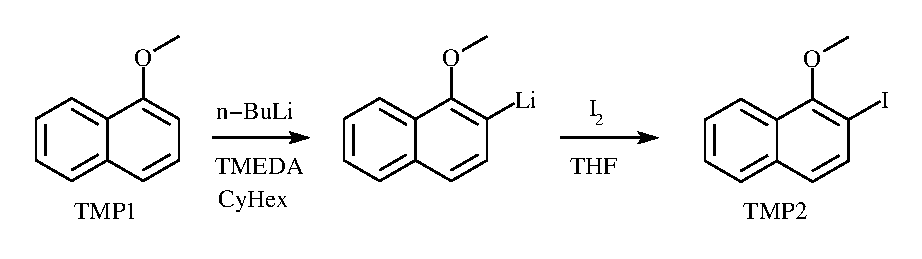
\includegraphics[width=.7\textwidth]{sc/mon-moni.eps}}
  \caption{\\ The iodination of \cmpd+{mon}.\label{sc:mon-moni}}
  \end{SCfigure}
  \paragraph{Strategy Synthesis}
    An ortho-directed metalation with \n-butyl\-lithium was used to selectively activate the 2 position of 1-methoxy\-naphthalene \cmpd+{mon} \cite{Shirley1969}. The metalation was performed in hydrocarbon solvent and in presence of TMEDA, likely useful to disaggregate \n-butyl\-lithium hexamers. Then iodine in ethereal solvent was added directly into the reaction mixture to obtain 2-iodo-1-methoxy\-naphthalene \cmpd+{moni} following the procedure from \citet{Cox1992}. 

  \paragraph{Results and Characterization}
    The product was isolated by column chromatography, obtaining a yield of 40~\%. 

    $^1$H-NMR and $^{13}$C-NMR spectra data are reported in Subsection \ref{sec:sperimentale-moni}, $^1$H-NMR spectrum is reported in Figure \ref{sp:moni}.
    In $^1$H-NMR of 2-iodo-1-methoxy\-naphthalene \cmpd+{moni} we can clearly distinguish peaks from the different groups of protons. The singlet at 4.03 ppm belongs to the protons of the methoxy substituent. Assignation of the signals can be simplified comparing our spectrum with the known spectrum\footnote{Source of the known spectra of $\alpha$-meth\-oxy-napthalene: \emph{Spectral Database for Organic Compounds SDBS}} of $\alpha$-meth\-oxy-napthalene. A striking difference is the absence in spectrum of \cmpd+{moni} of a rather shielded aromatic peak that was assigned to the proton in $\beta$ position next to the meth\-oxy group in $\alpha$-meth\-oxy-napthalene. 
    This confirms that the iodination reaction worked as expected. Comparing with the known spectra we can assign the peak at 8.21~ppm to the proton in position 2 and half of the peak at 7.82~ppm to the proton in position 5%com'era prevedibile non è piaciuto alla prof nemmeno questo "mezzo picco"
. The more shielded aromatic signal was assigned to hydrogen in position 7 in \emph{para} to the donating methoxy group. It's reasonable that signals from H in positions 3 and 4 are together and they don't move from \cmpd+{moni} to \cmpd+{dhn} from this consideration follows these protons generate the multiplet signal at 7.50 - 7.63~ppm. As a consequence the second proton at 7.82~ppm is assigned to the proton in position 8, de\-shielded by the vicinal iodine atom. 
    
%ALLA PROF, ERA SCONTATO, NON E' PIACIUTA LA NUMERAZIONE STRAVAGANTE CHE ABBIAMO USATO (che era quella data automaticamente da MestreNova...)

%Then the two doublets at 8.21 and 7.33~ppm are the signals of the protons on the substituted ring, where the most de\-shielded is that one in 4 and the other signal belongs to the proton in 3. The triplet is the signal of protons 5 and 8 and multiplet belongs to protons 6 and 7.
%secondo me è una cazzata.... questa sembra non tornare.
%  i due doppietti hanno J diverse e il tripletto ha la stessa J di uno dei due, come anche alcuni picchi del multipletto
%che quello sia un quartetto più un tripletto? e come potrebbero essere?

% Ragionamenti by AnreaLeo
%  confronto uno per uno, si può partire da quello dell'alfa metossi naftalene che trovi qui http://riodb01.ibase.aist.go.jp/sdbs/cgi-bin/img_disp.cgi?disptype=disp3&imgdir=hsp&fname=HSP40343&sdbsno=1333 ma secondo me può andare bene anche fare il confronto fra i due composti così come dico sotto 
% 
%  il segnale a 8.20 (1) rimane più o meno nel solito posto in entrambi gli spettri, quindi non può essere sull'anello sostituito, quindi e H2, deschermato dalla vicinanza dell'ossigeno. 
% 
% non devono cambiare posto anche 3, 4 e 5. confontando si vede che il picco a 7.55 (1) resta fermo e conta per due protoni, quindi sono 3 e 4 che "vedono" la stessa situazione di J. del tripletto a 7.8 (1) resta solo un "doppietto" a 7.9 (2) e questo è 5, quindi 7.8 del primo composto è dato dalla  sovrapposizione di due segnali diversi (5 e uno fra 7 e 8) 
% 
% Il segnale che era a 7.3 (1) si sposta tantissimo, quindi è uno dei due sull'anello sostituito perchè risente del cambiamento di sostituente. Molto probabilmente è 8 che risente dello schermo dovuto agli elettroni dello iodio. il segnale di 7 allora era sovrapposto a quello di 5. 
% 
% nel prodotto di coupling resta da determinare chi dei due doppietti è 7 e chi è 8. Per 8 la situazione cambia drasticamente (da iodio a naftile, come vicini). per 7 un po' meno. però non trovo una spiegazione plausibile per dire perchè 7 è a 7.6 (2) e 8 a 7.7 (2). 



\subsection{Coupling Using Palladium}
  \begin{SCfigure}[][ht]
    \cmpdref-{moni}
    \cmpdref-{schifo}
    \centering{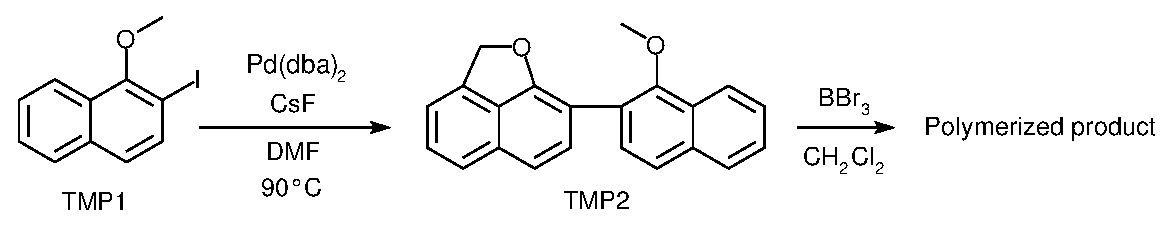
\includegraphics[width=.8\textwidth]{sc/moni-polimero.eps}}
  \caption{\\ The failed Pd homocoupling of \cmpd+{moni}.\label{sc:moni-polimero}}
  \end{SCfigure}

  \paragraph{Strategy Synthesis}
    At first a palladium catalyzed homo\-coupling was performed following the procedure from \citet{Seganish2005}. In this article also demanding substrates like \emph{ortho}-substituted and activated%or deactivated?? - Leo. Nono è più difficile couplare roba elettronricca come la nostra.
 aryls were coupled. 1-iodo-2-methoxy-benzene was reported to be successfully homo\-coupled using palladium(0) catalyst (10~\%) and TBAF in DMF. CsF (10~eq) is also indicated as a suitable and cheaper source of fluoride, so we used CsF.

  \paragraph{Results and Characterization}
    The reaction mixture was extracted and purified using column chromatography. The product was subjected to the deprotection treatment with \ce{BBr3} to afford an unexpected polymerized product. $^{13}$C-NMR spectrum peaks data for the coupling product is reported in Subsection \ref{sec:sperimentale-schifo}, it shows 22 signals, revealing the undesired asymmetric nature of the product. This substance was identified using GS-MS analysis and resulted to be an unexpected fused furan \cmpd+{schifo}. This molecule was reported from \citet{Dyker1994} as the result of a similar reaction
\footnote{Reaction conditions to obtain \cmpd+{schifo} from \cmpd+{dmon}: 2~mmol of \cmpd+{moni}, 8~mmol of \ce{K2CO3}, 2~mmol of tetra-\n-butylammonium bromide, 53~$\mu$mol of \ce{Pd(OAc)2}, 10~mL of DMF in sealed tube was stirred under \ce{N2} at \SI{100}{\celsius} for 3 days. After dilution with water the reaction was extracted with ether. The extracts were filtered through silica gel and the solvent removed by evaporation. The product was purified by flash chromatography (silica gel, \ce{Et2O}:hexane 1:20). Yield 71~\%. Procedure from \citet{Dyker1994}.}.
  
  \begin{SCfigure}[][ht]
    \cmpdref-{moni}
    \cmpdref-{intermedio1}
    \cmpdref-{schifo}
    \centering{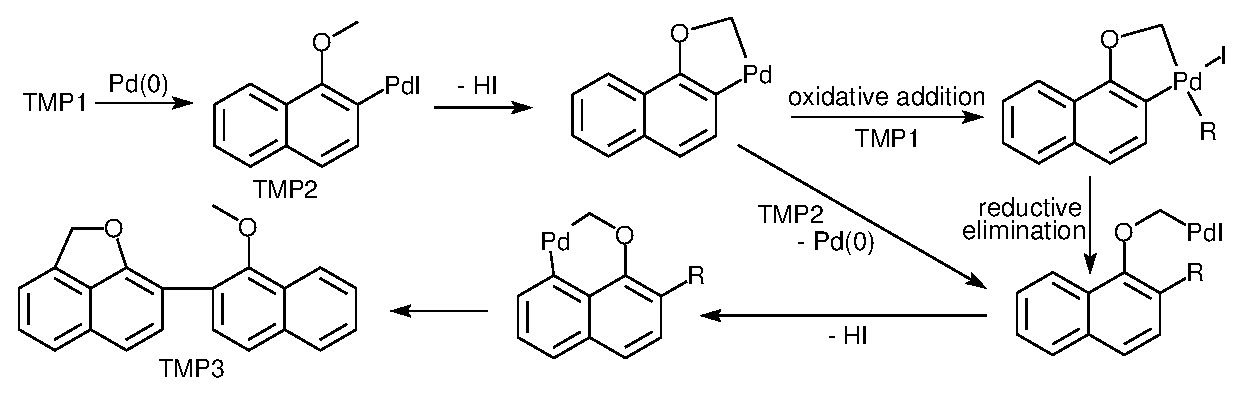
\includegraphics[width=1\textwidth]{sc/formazione-schifo.eps}}
  \caption{\\ The reported mechanism for the homo\-coupling - C-H activation at methoxy group domino process \cite{Dyker1994}.\label{sc:formazione-schifo}}
  \end{SCfigure}

\subsection{Ullmann Reaction}
  \begin{SCfigure}[][ht]
    \cmpdref-{moni}
    \cmpdref-{dmon}
    \cmpdref-{dhn}
    \centering{
\includegraphics[width=.8\textwidth]{sc/moni-dhn.eps}}
  \caption{\\ The Ullmann homo\-coupling of \cmpd+{moni}.\label{sc:moni-dhn}}
  \end{SCfigure}

  \paragraph{The Coupling}
    The Ullmann reaction is a 111 years old reliable solvent-free coupling which involves a more than stoichiometric amount of metallic copper and, in its traditional version, very high temperatures (\textgreater\SI{200}{\celsius}). This reaction allows to homo\-couple an aryl iodide. 
    \emph{Our laboratory group didn't perform the Ullmann reaction} and the desired 1,1'-dimethoxy-2,2'-bi\-naphthalene \cmpd+{dmon} was shared with us by another lab group. They synthesized the molecule following a procedure from \citet{JR9310001265}: copper (3 equivalents), a catalytic amount of iodine and 1,1'-dimethoxy-2,2'-bi\-naphthalene \cmpd+{dmon} were heated at \SI{170}{\celsius} for 5 hours.% long.

  \paragraph{De\-protection}
    In the end the deprotection using \ce{BBr3} in di\-chloro\-methane afforded the desired 1,1'-di\-hydroxy-2,2'-bi\-naphthalene \cmpd+{dhn} after quenching with water \cite{McOmie1968}.

  \paragraph{Results and Characterization}
    $^{1}$H-NMR spectrum of 1,1’-di\-hydroxy-2,2’-bi\-naphthalene \cmpd+{dhn} is reported in Figure \ref{sp:dhn}.
    Peaks data from $^{1}$H-NMR and $^{13}$C-NMR spectra are reported in Subsection \ref{sub:sperimentale-dhn}.
    
    Both $^{1}$H-NMR and $^{13}$C-NMR spectra show the symmetric nature of the compound, having few clear signals.
    
    Signals from protons in positions 2, 3, 4 and 5 (and equivalent protons 17, 18, 19, 20) were assigned as in the spectrum from 2-iodo-1-methoxy\-naphthalene \cmpd+{moni}. % Proton in position 8 is now less de\-shielded compared to 2-iodo-1-methoxy\-naphthalene \cmpd+{moni}.
    Signals from protons in positions 7 and 8 were difficult to assign. 


% Ragionamenti by AnreaLeo
%  di iodrossinaftalene anche qui ricorro al giochino del confronto (ora sono più che autorizzato a farlo) 
% 
% 2, 3, 4 e 5 rimangono quasi invariati anche dopo la demetilazione 7 e 8 si sono spostati e uno si è sovrapposto a 3 e 4, ma la forma si distingue senza problemi. si nota che 2 è più deschermato, dovuto al cambiamento metossi-ossidrile, 3, 4 e 5 hanno avuto pochi cambiamenti, ma 7 e 8 si sono spostati parecchio, probabilmente il cambiamento di geometria fra prima e dopo è abbastanza consistente. adesso i legami a idrogeno dovrebbero favorire due conformazioni enantiomeriche (dando un racemo).  e qui si sgama chi è 7 e 8 nel metossi e nell'idrossi binaftile: i due picchi si spostano, ma uno di più, quindi è più vicino all'altro OH. e quello più vicino è 8. quindi adesso a 7.4 c'è 8 e a 7.6 c'è 7. nel metossi erano rispettivamente a 7.62 e 7.7 
% 
% osservazione: sovrapponendo gli spettri si vede chiaramente che il nostro di metossi era in parte deprotetto perchè il segnale a 7.4 di 8 c'è in tutti e due gli spettri esattamente nello stesso posto 

\section{Synthesis of Phosphite Ligand}


  \paragraph{Strategy Synthesis}
  \begin{SCfigure}
    \cmpdref-{amda}
    \cmpdref-{dhn}
    \cmpdref-{legante}
    \centering{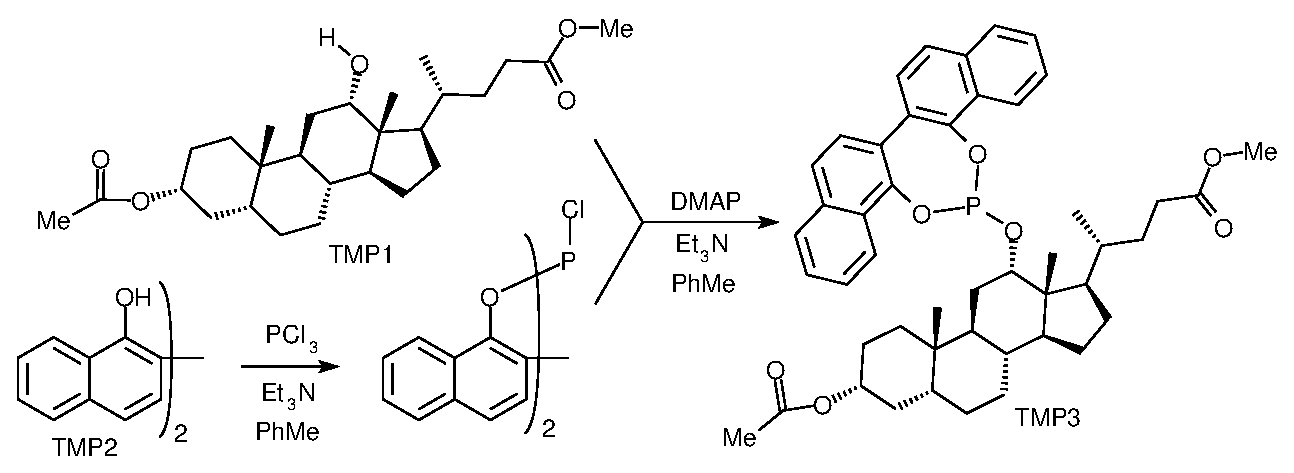
\includegraphics[width=1\textwidth]{sc/amda-dhn-legante.eps}}
    \caption{\\ Joining the aromatic and aliphatic part of the ligand \cmpd+{legante}.\label{sc:amda-dhn-legante}}
  \end{SCfigure}
  In order to join the aromatic and the aliphatic part of the ligand \cmpd+{legante} a two step synthesis was performed: the bi\-naphthol \cmpd+{dhn} was converted in bi\-naphthyl chloro\-phosphite that was subsequently reacted with the available alcoholic group of the protected de\-oxy\-cholic acid \cmpd+{amda}. 
  \ce{PCl3} was added to a solution of 1,1'-di\-hydroxy-2,2'-bi\-naphthalene \cmpd+{dhn}, the hydrochloric acid formation was prevented adding \ce{Et3N} and the solid quaternary ammonium salt formed was filtered maintaining the system under inert atmosphere. The obtained reaction mixture was added to the protected de\-oxy\-cholic acid \cmpd+{amda} in the presence of \ce{Et3N} and 4-dimethyl\-amino\-pyridine (DMAP). DMAP helps the $\mathrm{S_N}2$ etherification substituting the chlorine atom and behaving as a better leaving group.  
  There is risk of oxidation of the resulting phosphite in the purification while running on silica gel column, so the eluent was chosen to elute fast the product.

%fosfito colonna veloce x non avere ossidazione
  \paragraph{Results and Characterization}
    The reaction mixture was filtered and purified by flash chromatography to produce a 5~\% yield in pure ligand \cmpd+{legante}.
    
    $^{1}$H-NMR spectrum of phosphite ligand \cmpd+{legante} is reported in Figure \ref{sp:legante}. We can clearly recognize the presence of the peaks belonging to the de\-oxy\-cholic part of the molecule and the sharp aromatic signals of the bi\-naphthylic side. Correlation of the signals from the aliphatic part was done similarly to the previous assignation of spectrum of protected de\-oxy\-cholic acid \cmpd+{amda}. The unique interesting difference is the enhanced de\-shielding of the proton in position 12 caused by the conversion of the group in $\alpha$ from hydroxylic to phosphite.
    The aromatic part of the spectrum is more dense of peaks than in spectrum of 1,1'-di\-hydroxy-2,2'-bi\-naphthalene \cmpd+{dhn} maybe due a loss in symmetry. 
    
%    From the $^{1}$H-NMR spectrum of the ligand we can clearly see the presence of the five singlet peaks belonging to the methyl groups of the de\-oxy\-cholic part of the molecule and the sharp aromatic signals of the bi\-naphthylic side.
    


% Ragionamenti by AnreaLeo
% legante. 
% 
% per la parte aromatica ci si può affidare solo al fatto che l'integrazione è coerente con quello che ci si aspetta, che si è persa la simmetria del sistema molto probabilmente i segnali a 8.5 e 8.6 sono i protoni 2 e 2' del binaftile che sono stati separati dall'ambiente chiarale (sono rivolti verso la cavità) degli altri segnali aromatici si dice poco. al massimo che si notano molte J uguali (le J dopo la coordinazione non cambiano) ereditate dal diidrossinaftalene. le posizioni sono cambiate molto. l'unica uguale è il CDCl3.... 
% 
% per la parte alifatica è meno difficile. confrontando con il derivato biliare si nota un generale spostamento verso ppm pià bassi (campo alto o basso? non ricordo). segnali diagnostici dello spostamento sono i metili: tutti sono spostati tranne quello sul C20, che è più o meno nella stessa posizione, così come il protone a 4.7. quello a 4.00 è stato spostato a 4.25. il metile sul C20 e il protone sul C3 quasi non risentono della presenza del binaftile, mentre il protone sul C12 viene addirittura  deschermato. Questo effetto dovrebbe essere il risultato dell'azione contemporanea del fosforo e del binaftile. 
% 
% da quel che ho capito hai fatto due spettri del legante, uno intero e uno tagliato. io preferisco quello intero, perchè in quello tagliato si vede troppo bene i segnali della parte deossicolica 

%"si vede troppo bene i segnali della parte deossicolica" gigalol




    A series of variable temperature $^{31}$P-NMR spectra of the ligand \cmpd+{legante} were performed. The scope was studying the broadening of the peak  due to the slower motion of atrop\-isomerization reaching very low temperatures. The spectra were recorded without shimming nor locking using non-deuterated toluene and phosphoric acid as an external reference. Only a very slight broadening of the peak was observed reaching \SI{-90}{\celsius} instead of the expected decoalescence in two separated peaks. 
    Probably this means that the interconversion between M and P conformers of the bi\-naphthyl group is still too fast at this temperature (hence,  the isomerization barrier is very low). An alternative explanation is that the atro\-poisomeric conformation induction of the de\-oxy\-cholic ester is so strong that our ligand \cmpd+{legante} was present in only one conformation, already at room temperature.

    The combined information gained from this $^{31}$P-NMR and $^{1}$H-NMR spectra of \cmpd+{dhn} and of \cmpd+{legante} show that the homocoupling of the naphthylic product proceeded as intended and that the purified ligand is composed only of the compound we were looking for and not by a mixture of compounds.
    In the spectrum in Figure \ref{sp:dhn} the two doublets at 7.40 ppm and at 7.59 ppm (this one is overlapping other signals, but is higher than those and so recognizable) imply that the substituents on the naphthalene are on the same ring and either in positions 1 and 4 or 1 and 2. In the spectrum of the ligand we can see that the ratio between the bi\-naphthylic part and the de\-oxy\-cholic one is almost 1:1 and from the $^{31}$P-NMR spectra we know that there is only one species of phosphorus.
    The information so gained are compatible with a compound with a bi\-naphthylic group in which the oxygens both bond the P atom and this form a phosphate with the de\-oxy\-cholic ester. The only way to achieve this structure is to have substituents on each naphthylic unit in position 1 and 2, that is, the ligand we want to prepare.

    In the circular dichroism spectrum we could expect the presence of an exciton couplet (due to the coupling of the oscillators along the long axis of the naphthylic groups), but the spectrum shows a series of weak peaks whose wavelengths correspond to positions of the peaks in UV-vis spectrum. %This observation gives rise to doubts about the presence of the exciton couplet. %In particular, around 200~nm the wavelenghts of the Cotton Effects are closing matching those of the peaks in the UV-vis spectrum and is not easy to determine if the shape of the CD spectrum is due to two different CE of opposite sign or to an exciton couplet.
    A waveform similar to a exciton couplet can be observed in the short wavelength part of the spectrum. 

%  \paragraph{UV-vis and Circular Dichroism spectra}

% temp. variabile non si splitta, vuol dire che < 10 kcal/mol \cite{Facchetti2006}
% in toluene non deuterato
% no shim no lock
% rif acido fosforico
% 200MHz
% 166ppm

  \paragraph{Computational study}
    In order to understand the circular dichroism spectrum and to verify the stereo\-chemistry of the bi\-naphthylic group a computational study was performed. The ligand \cmpd+{legante} geometry was optimized in free space starting from a M (R$_a$) atrop\-isomer without performing any conformers search. Using data provided by the semi-empirical calculation is possible to obtain an estimation of 42 degrees for the dihedral angle between the two bi\-naphthylic units. Then a time-dependent DFT calculation gave a simulation of the circular dichroism spectrum. 
    This computation was performed on the whole ligand using Gaussian\textsuperscript{\textregistered} development version, B3LYP method, 6-311+g(d) basis set considering 20 states (thanks to Lorenzo for this calculation). The resulting UV-vis spectrum isn't too different from the experimental one. The calculated CD spectrum shape is very similar to the experimental one, but is redshifted by 40~nm. This discrepancy in results was not understood, nevertheless was speculated that the real conformation of the \emph{atropos} bi\-naphthylic group is M (R$_a$). Calculated HOMO and LUMO were reported, Figures \ref{sp:lumo} and \ref{sp:homo}.



\section{Conjugate Addition to nitro\-cyclohexene}
  The asymmetric reaction of addition of phenyl\-boronic acid to electron-poor alkenes have been applied with high enantio\-selectivity to various substrates like conjugate ketones, esters, amides and nitro\-alkenes.
  \begin{SCfigure}
    \cmpdref-{pba}
    \cmpdref-{nc}
    \cmpdref-{ncb}
    \centering{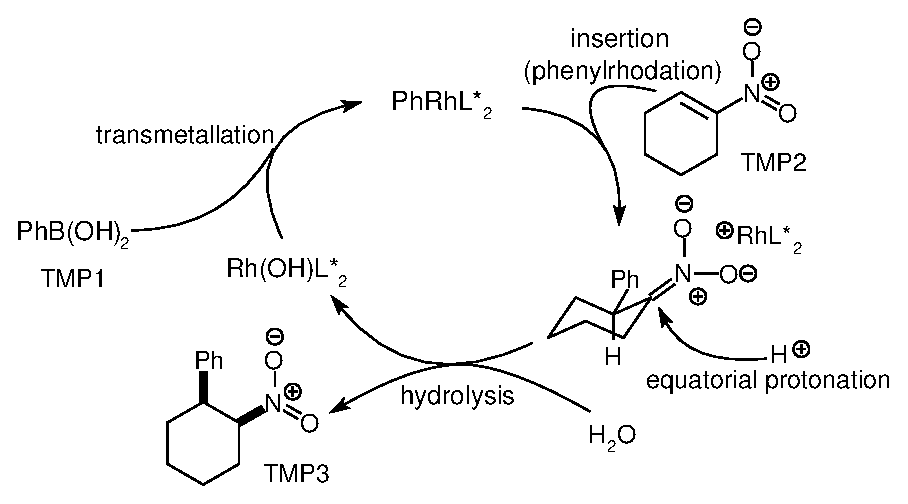
\includegraphics[width=0.8\textwidth]{sc/meccanismo.eps}}
    \caption{\\ An hypothesis on the mechanism of the conjugate addition. L* = \cmpd+{legante}. Loosely based on \cite{Hayashi2000} and \cite{Hayashi2002}.\label{sc:meccanismo}}
  \end{SCfigure}

\paragraph{Rhodium Catalyst}
  The rhodium(I) catalyst was needed to perform the conjugate addition object of this study. Dimeric rhodium complex \ce{[RhCl(C2H4)2]2} and phosphite ligand \cmpd+{legante} in the presence of an aqueous base were used to form the catalyst in situ. Ethylene is easily replaced by the phosphite ligand to produce [RhCl(L$^\ast$)$_2$]$_2$, then the aqueous base removes the chloride ion forming [Rh(OH)(L$^\ast$)$_2$]$_2$ which is more active towards the rate-determining transmetalation step of the hypothesized catalytic cycle in Figure \ref{sc:meccanismo}. 
  The choice of the source of rhodium is important: for example starting from \ce{Rh(acac)(C2H4)2}, the reaction would have required higher temperatures (bringing to the hydrolysis of phenylboronic acid to give benzene) due to the more difficult transmetalation \cite{Hayashi2002}. 
  The rhodium-ligand equivalents ratio was chosen to be 1:2 as reported to form the more active disubstituted complex \cite{Facchetti2009}. According to the authors it is also possible that sterically hindered ligands cannot form disubstituted complexes. But this hypothesis requires further investigation.
%\paragraph{Addition of Boronic Acid to Nitro Cyclohexene}%Reaction Environment}
  \paragraph{Strategy Synthesis}
    The conjugate addition was performed one-pot with the preparation of the catalyst.
    Boronic acids are stable to water and air, easy to prepare and often provided from commercial suppliers. By the way in this reaction boronic acid has to be used over-stoichiometric due to a side reaction of proto\-de\-boronation.
    This procedure wasn't reported in the literature, we obtained it from Varsha Katkar Jumde, post-doctoral researcher in Prof. Iuliano's laboratory.     
    The presence of an aqueous base is also useful for the quaternization of the boronic acid, promoting the transmetalation.


\paragraph{Results and Characterization}

GC analysis (Figure \ref{sp:gc}) showed poor conversion of the initial reagent into the addition product (17~\%) and the formation of 4 products: \emph{cis} (1\rS,2\rS), (1\Rs,2\Rs) and \emph{trans} (1\rS,2\Rs), (1\Rs,2\rS) [(1{\slshape ?},2{\slshape ?})-2-nitro-cyclo\-hexyl]benzene \cmpd+{ncb}.
\emph{Trans} diastereomer resulted to be the prevalent compound with a diastereo\-meric excess of 25~\%. Chiral HPLC analysis (Figure \ref{sp:hplc}) allowed to determine enantiomeric excess of the isolated \emph{trans} product as 60~\%. 

$^{1}$H-NMR spectrum, reported in Figure \ref{sp:prodotto}, is very crowded: we can recognize various molecules. The highest signals seem to indicate the presence of un\-reacted 1-nitro\-cyclo\-hexene \cmpd+{nc}: ratio of areas of main peaks from Figure \ref{sp:prodotto} is compatible with 1-nitro\-cyclo\-hexene \cmpd+{nc}\footnote{The ratio of area of main peak in aromatic zone over area of peaks from cyclohexane ring is 1:8, compatible with \cmpd+{nc} and incompatible with \cmpd+{ncb}.} moreover we can recognize \cmpd+{nc} comparing with the $^1$H-NMR spectrum supplied by the seller\footnote{The $^1$H-NMR spectrum of 1-nitro\-cyclo\-hexene \cmpd+{nc} in \ce{CDCl3} is provided by Sigma-Aldrich\textsuperscript{\textregistered}.}. 
We can see also some phosphite ligand \cmpd+{legante}. It is possible that some de\-protection of the phosphite ligand occurred in presence of KOH and water at high temperatures but we can't demonstrate this studying the $^{1}$H-NMR spectrum. There are no peaks from phenyl\-boronic acid, maybe it was removed by purification or by hydrolysis. Peaks from the product are very weak and of uncertain assignation. 


% Ragionamenti by AnreaLeo

% prodotto di addizione 
% 
% hai già fatto te l'assegnazione. i segnali del legante sono ben distinguibili dagli altri (il malloppone fra gli aromatici e quello dell'acido biliare) però non so come hai fatto l'assegnazione del nitrocicloesene.... "sapendo che la conversione è del 17% possiamo assegnare con tranquillità i segnali più intensi al nitrocicloesene"... 
% 
% altrimenti si può dire che il picco molto intenso fra gli aromatici e la medesima intensità di altri picchi nell'area degli fanno supporre l'appartenenza a uno stesso composto. non può essere acido fenil boronico perchè non ha segnali alifatici, non può essere il prodotto di addizione perchè avrebbe un segnale più complesso nella zona degli aromatici e la presenza di protoni alifatici molto dechermati (intorno a 3-4 ppm a causa della presenza simultanea del gruppo fenilico e del nitro. Inoltre se riesci a vedere qualcosa con le J sarebbe meraviglioso. comunque c'è sempre l'integrazione, che approssima fin troppo bene ai protoni del nitrocicloesene (tre gruppi di due protoni, un protone solitario e un tripletto (che si vede) per un protone negli aromatici (J=4.20 picchi a 7.300, 7.315 e 7.330) poi ci sono i picchi piccoli che si possono attribuire al prodotto di addizione ma se possibile eviterei di parlarne. 
% 
% da notare c'è che, nonostante si riconosca la posizione (anche relativa)  e la forma dei picchi, quasi tutti sono spostati (un po' in qua e un po' in là) Azzarderei a causa della complessazione col Rh che ha indotto un po' di deformazione dei gruppi del legante



%\paragraph{$^{1}$H-NMR Spectra}
%ma c'è? no? sì ma fa schiiiifo c'è pure il legante presente





